\subsection{Modèle de données}
\begin{frame}{Conception}{Modèle de données}
\begin{block}{Modèle original}
\begin{center}
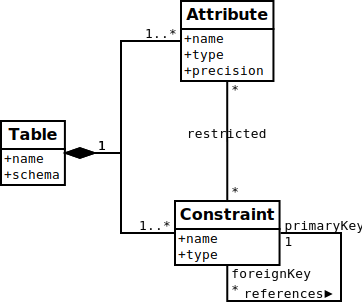
\includegraphics[width=0.5\textwidth]{files/diag_class_origine}
\end{center}
\end{block}
\end{frame}

\begin{frame}{Conception}{Modèle de données}
\begin{block}{Modèle réel}
\begin{center}
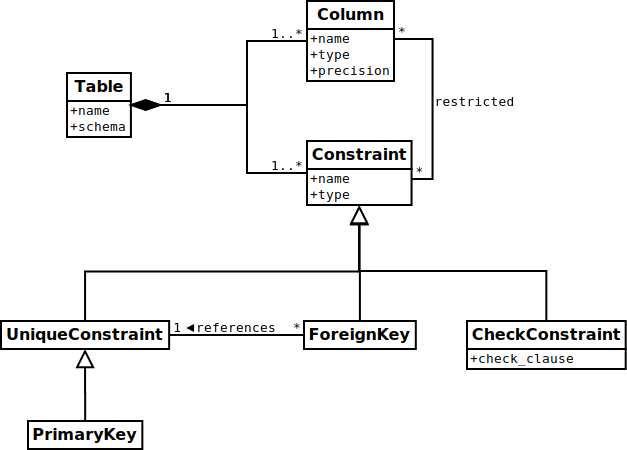
\includegraphics[width=0.8\textwidth]{files/diag_class_ameliore}
\end{center}
\end{block}
\end{frame}

\subsection{Compatibilité}
\begin{frame}{Conception}{Compatibilité}
\begin{block}{Configuration d'un SGBD}
	\begin{itemize}
	\item Un fichier de configuration général
	\item Des fichiers de mapping
	\end{itemize}
\end{block}
\begin{block}{Généricité des types}
Gestion de la correspondance de types pour chaque SGBD.
\end{block}
\end{frame}

\def\itemizeGUI{
\begin{itemize}
	\item User-Friendly
	\item Permet un affichage dynamique
	\item Plus intuitif
	\end{itemize}
}

\def\itemizeCLI{
	\begin{itemize}
	\item KISS
	\item Légèreté
	\item Interopérabilité
	\item Surcouche GUI possible
	\end{itemize}
}

\subsection{IHM}
\begin{frame}{Conception}{Visualisation}
\begin{columns}[t]
\begin{column}{0.5\textwidth}
	\only<1>{
	\begin{block}{CLI}
	\textit{Command Line Interface}
	\itemizeCLI
	\end{block}
	}
	\only<2>{
	\begin{exampleblock}{\emph{CLI}}
	\textit{Command Line Interface}
	\itemizeCLI
	\end{exampleblock}
	}
\end{column}
\begin{column}{0.5\textwidth}
	\only<1>{
	\begin{block}{GUI}
	\textit{Graphical User Interface}
	\itemizeGUI
	\end{block}
	}
	\only<2>{
	\begin{alertblock}{\sout{GUI}}
	\textit{\sout{Graphical User Interface}}
	\itemizeGUI
	\end{alertblock}
	}
\end{column}
\end{columns}
\end{frame}

\subsection{Visualisation}

\begin{frame}{Conception}{Visualisation}
\begin{columns}[t]
\begin{column}{0.4\textwidth}
	\begin{block}{Librairies}
		\begin{itemize}
		\item Graphviz
		\item JUNG
		\item Grappa
		\end{itemize}
	\end{block}
\end{column}
\pause
\begin{column}{0.6\textwidth}
	\begin{exampleblock}{$\Rightarrow$ Graphviz}
		\begin{itemize}
		\item Basée sur DOT
		\item Simplicité d'intégration
		\item Possibilité de nœuds complexes
		\item Génération d'image
		\end{itemize}
	\end{exampleblock}
\end{column}
\end{columns}
\end{frame}